\chapter{Неэргодичность спинового стекла}\label{ch:ch4}

\section{Линии нестабильности}

\begin{figure}[!ht]
	\centering
	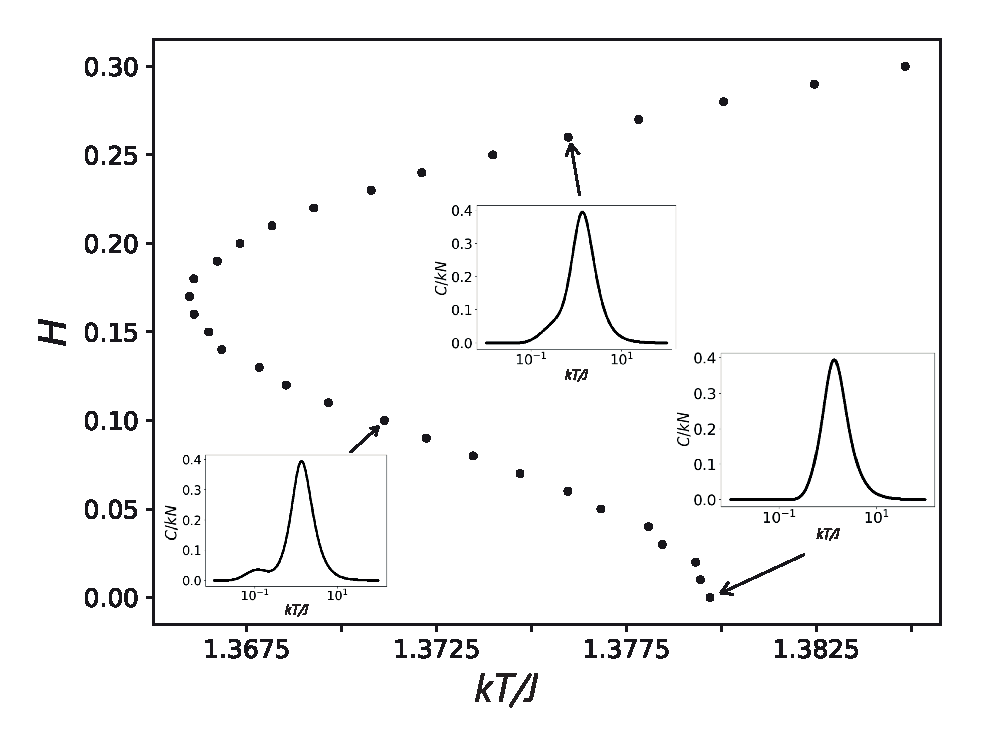
\includegraphics[width=0.8\linewidth]{Ginsburg_T_aver1.eps}
	\caption{Линия нестабильности системы конечного числа спинов Изинга в модели Эдвардса-Андерсона во внешнем магнитном поле. На вставках приводится температурное поведение теплоемкости во внешнем магнитном поле для систем $P_{+}=0.5$.}
	\label{fig:Stable_line}
\end{figure}

\begin{figure}[!ht]
	\centering
	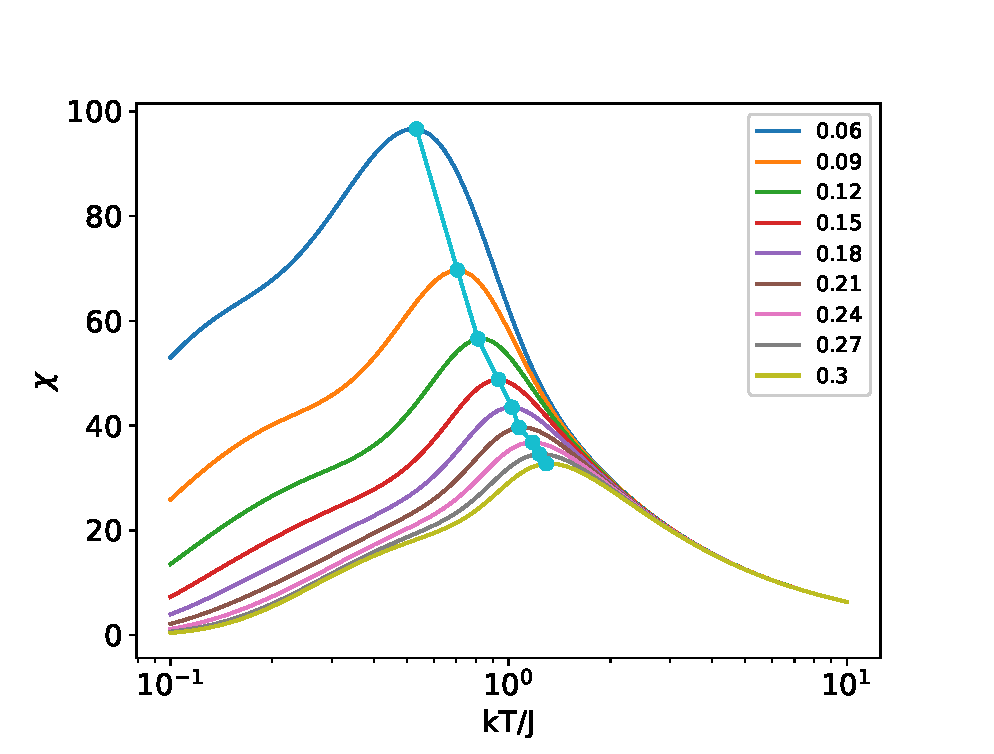
\includegraphics[width=0.8\linewidth]{Chi(kT)_J0_8.eps}
	\caption{Температурное поведение магнитной восприимчивости во внешнем магнитном поле для систем $P_{+}=0.5$ количеством частиц $N = 8 \times 8$. Значения модуля напряженности внешнего магнитного поля приведены на вкладке}
	\label{fig:Chi(kT)_J0_8.eps}
\end{figure}

Как отмечалось в работе \cite{takzei1984} на фазовой диаграмме $H-T$ можно наблюдать линию нестабильности Алмейды-Таулеса. В работе \cite{takzei1984} эти данные получены при анализе намагниченности при разных режимах проведения эксперимента. Наши результаты строгих вычислений показывают, что в малых полях наблюдается понижение средней температуры максимума теплоемкости с ростом малых значений внешнего магнитного поля $0.0<H<0.3$ в единицах обменных интегралов, см. рисунок \ref{fig:Stable_line}. Малыми мы считаем значения напряженности внешнего магнитного поля $H$ по отношению к напряженности полей взаимодействия между спинами. Небольшие изменения в низкотемпературном поведении теплоемкости возможно связаны с открытыми граничными условиями.


Данная линия получена по данным температурного поведения максимума теплоемкости. Данные по температурам максимумов теплоемкостей были усреднены по всем образцам с одинаковым $P_{+}$, в т.ч. на рисунках \ref{fig:Diag}, \ref{fig:Diag1} и \ref{fig:Diag4}. Оказалось, что для $P_{+}=0.5$ при увеличении модуля напряженности внешнего магнитного поля до $H<0.05$ в единицах $J$ температура максимума теплоемкости остается фиксированной. 

Можно предположить, что энергия Зеемана действует как хаотизирующий фактор, который приводит к понижению температуры максимума теплоемкости. В относительно высоких внешних магнитных полях $H>0.23$ температура максимума теплоемкости начинает расти, также, как в ферромагнитной модели из за эффекта опрокидывания спинового стекла.

Расчеты магнитной восприимчивости в поле произведены по формуле 
\begin{equation}
	\chi(T)=\frac{\partial \langle M \rangle (T)}{\partial T}\bigg|_{h\rightarrow 0}=\frac{\langle M^2 \rangle-\langle M \rangle ^2}{k T^2},
	\label{eq:ct}
\end{equation}
где
\begin{equation}
	\langle M \rangle (T) =\frac{1}{Z}\sum_{t=1}^{\Omega}g_t M_t \exp\left\{-\frac{E_t-h M_t}{kT}\right\}
	\label{eq:ct}
\end{equation}
и
\begin{equation}
	\langle M^2 \rangle (T) =\frac{1}{Z}\sum_{t=1}^{\Omega}g_t M_t^2 \exp\left\{-\frac{E_t-h M_t}{kT}\right\}.
	\label{eq:ct}
\end{equation}


На рисунке \ref{fig:Chi(kT)_J0_8.eps} видно, что при увеличении модуля напряженности внешнего магнитного поля температура максимума магнитной восприимчивости снижается для образов $P_+=0.5$. Таким образом, строгое вычисление статистической суммы   конечного числа спинов Изинга фактически означает, что физика изучаемых систем для $P_+=0.5$, которые находятся в состоянии спинового стекла является равновесной. Для объяснения существования линии нестабильности на $H-T$-диаграмме не требуется привлечения таких понятий как ''неэргодичность'', ''ультраметричность топологии пространства долин'', ''необратимость'' и других.